\documentclass{article}
\usepackage[dutch]{babel}
\usepackage{graphicx}
\usepackage{float}
\usepackage{geometry}
\usepackage{fancyhdr}

\geometry{a4paper, top=3cm, bottom=3cm, left=2cm, right=2cm}

\title{Adviesrapport: Data-driven Business}
\author{Yujian Jiang, Max Jansen}
\date{July 2025}

\begin{document}

\maketitle

\begin{figure}
    \centering
    
\includegraphics[width=4cm]{prorail.png}
\end{figure}

\pagestyle{fancy}

\newpage
\tableofcontents

\newpage
\section{Inleiding}

\subsection{Achtergrond van het project}
Voor het vak DataDriven Business is ProRail naar de HU gekomen met de vraag of wij hulp kunnen bieden voor het DataLab. Het DataLab is een afdeling van ProRail, waar grote hoeveelheden data worden verzameld, die daarna geanalyseerd en verwerkt worden om verbeteringen toe te passen op het spoorwegnet. Het spoorwegnet is erg groot en er zullen altijd wel problemen opduiken van klein tot groot. Dit is voor iedereen erg vervelend. ProRail is daardoor veel bezig met het oplossen van de problemen en de kosten lopen daardoor ook op. Ook voor de reizigers is het vervelend. Die moeten omreizen en zullen zich ergeren als het herhaaldelijk optreedt. Het is dus van groot belang dat problemen snel en efficiënt worden opgelost om zowel kosten te besparen als de tevredenheid van de reizigers te behouden.

\subsection{Het belang van een snelle oplossing}
Het is belangrijk dat er snel gehandeld wordt. Daarvoor moet wel duidelijk zijn wat de problemen zijn en hoe lang die gaan duren, zodat er vooruit gepland kan worden om de minste vertragingen op te lopen. Als er bijvoorbeeld een storing is, moeten de planners weten hoe lang het ongeveer gaat duren voordat het opgelost is, zodat ze alternatieve routes kunnen plannen of vervangend vervoer kunnen regelen. Nu is er dus gevraagd of er hulp geboden kan worden bij het verduidelijken van de problemen. Er is gevraagd of het mogelijk is om te voorspellen hoe lang een storing gaat duren, zodat er op tijd en beter omheen gepland kan worden en de vertragingen zo beperkt mogelijk kunnen blijven.

\newpage
\section{Opdracht}

\subsection{Doel van de opdracht}
De opdracht die wij gekregen hebben, is om uit te zoeken of het mogelijk is om te voorspellen hoe lang een storing gaat duren. Dit willen ze gaan doen door gebruik te maken van een applicatie die dit kan voorspellen. Op dit moment is de applicatie er nog niet. Die gaan wij maken. Maar voordat we dat kunnen doen, moeten wij inzicht krijgen in het gehele proces. We weten namelijk niet hoe ze bij ProRail te werk gaan. Ook moet de data grondig doorgenomen worden. De data moet worden geanalyseerd, opgeschoond en voorbereid voor de modellen die de voorspellingen gaan doen. Dan moet de applicatie gemaakt worden. Hoe het eruit gaat zien, welk model er gekozen wordt, en hoe het gebruikt gaat worden. Als laatste moet er gedocumenteerd worden. Er moet een duidelijke uitleg zijn, en alles moet gerapporteerd worden. Omdat het proces behoorlijk groot is, gaan we het verdelen in verschillende delen, wat uiteindelijk een geheel moet vormen.

\subsection{Deelopdrachten}

\subsubsection{Business Understanding}
Het eerste deel is de Business Understanding, zodat ons duidelijk wordt waar wij onze taken moeten vervullen en hoe het proces loopt. We doen namelijk een opdracht voor een extern bedrijf waar wij nergens bekend mee zijn. Ons moet duidelijk worden wat er van ons allemaal gevraagd wordt. We moeten weten wie de stakeholders zijn, waar onze data vandaan komt, en wat de knelpunten zijn. Maar ook hoe hun hele proces loopt, hoe het bedrijf te werk gaat, wat onze rol is. Pas als wij snappen hoe ProRail werkt, kunnen wij een opdracht voor ze maken.

\subsubsection{Data}
Als het eenmaal duidelijk is wat we moeten gaan doen, is de volgende stap het begrijpen van de data. Zonder de data kunnen we namelijk geen voorspellingen maken. De data is erg ingewikkeld en verre van schoon. We hebben 139 kolommen met allemaal onduidelijke namen, die we uiteindelijk getrimd hebben naar 58 kolommen. Ook zijn er $\pm$ 900.000 rijen waarmee we werken, en er staan heel veel lege/verkeerde waarden in. Het is dus een zooitje. Nu is het belangrijk om te begrijpen wat alles is, wat eruit gefilterd mag worden en waarmee we doorgaan. Daarnaast moet er goed worden geanalyseerd, zodat er vervolgens drie modellen uitgewerkt kunnen worden.

\subsubsection{Modellen}
Als we eenmaal inzicht hebben in de data, kunnen we beginnen met het bouwen van modellen. Het doel hiervan is om voorspellingen te doen die het werkproces kunnen ondersteunen. We gaan meerdere modellen testen, zodat we kunnen bepalen welke het beste werkt voor onze situatie. Belangrijk is dat we goed uitleggen waarom we bepaalde keuzes maken, welke algoritmes we gebruiken, en hoe accuraat de modellen zijn. Elk model heeft zijn eigen voor- en nadelen, en moet goed geanalyseerd worden. Uiteindelijk kiezen we het model dat het meest betrouwbaar is en het beste past bij de voorspellingen die gemaakt moeten worden. Dit model wordt dan verwerkt in de applicatie.
 
\subsubsection{Applicatie}
Het belang van de opdracht is een werkende applicatie. Dit gaat namelijk gebruikt worden door het personeel in de meldkamer, waar de storingen verwerkt worden. Hier komt het hele project samen. De applicatie gaat een van de gekozen modellen bevatten die de voorspelling gaat doen. Die gecreëerd is uit de analyse van de data. Maar ook omdat we inzicht hebben gecreëerd voor het bedrijf. Ook kun je alle oude data terugvinden om te kijken hoe de oude storingen waren, maar ook hoe lang het duurde voordat ze waren opgelost.

\subsubsection{Documentatie}
Om het project af te ronden is er goede documentatie nodig. Je kunt wel een werkend product neerzetten, maar als het niet duidelijk is hoe het gebruikt moet worden, kom je niet ver. Er wordt een duidelijke uitleg verwacht van hoe de applicatie gebruikt moet worden, maar ook hoe het model tot stand gekomen is. Er moet namelijk wel een goede reden zijn om geld en tijd te investeren in deze applicatie.
 
\newpage
\section{Business Understanding}

\subsection{Proces}
De eerste stap in het project is het in kaart brengen van het probleem en de oplossing waar we naartoe moeten werken. Om het probleem in kaart te brengen zijn wij druk bezig geweest met de mensen van ProRail om alles in kaart te brengen. Het proces begint wanneer iemand (de melder) een probleem opmerkt en contact opneemt met de meldkamer. De meldkamer zoekt vervolgens een aannemer die beschikbaar is en belt deze op. Zodra de aannemer onderweg is, maakt hij een prognose van het probleem. Op basis daarvan wordt bepaald of de treindienstregeling moet worden aangepast. Als dat zo is, wordt de planner op de hoogte gebracht. De aannemer komt aan op locatie en lost het probleem op. Tijdens dit hele proces worden belangrijke gegevens vastgelegd, zoals de oorzaak, locatie en duur van de storing. Zodra het probleem is opgelost, communiceert de meldkamer dit terug naar de betrokken partijen. De aannemer vertrekt en als alles in orde is, worden de treinen weer hervat. Dit hele proces is belangrijk om te snappen, omdat wij hierdoor weten op welk moment er welke data beschikbaar is, en waar onze applicatie het meest van waarde kan zijn.

\begin{figure}[H]
    \centering
    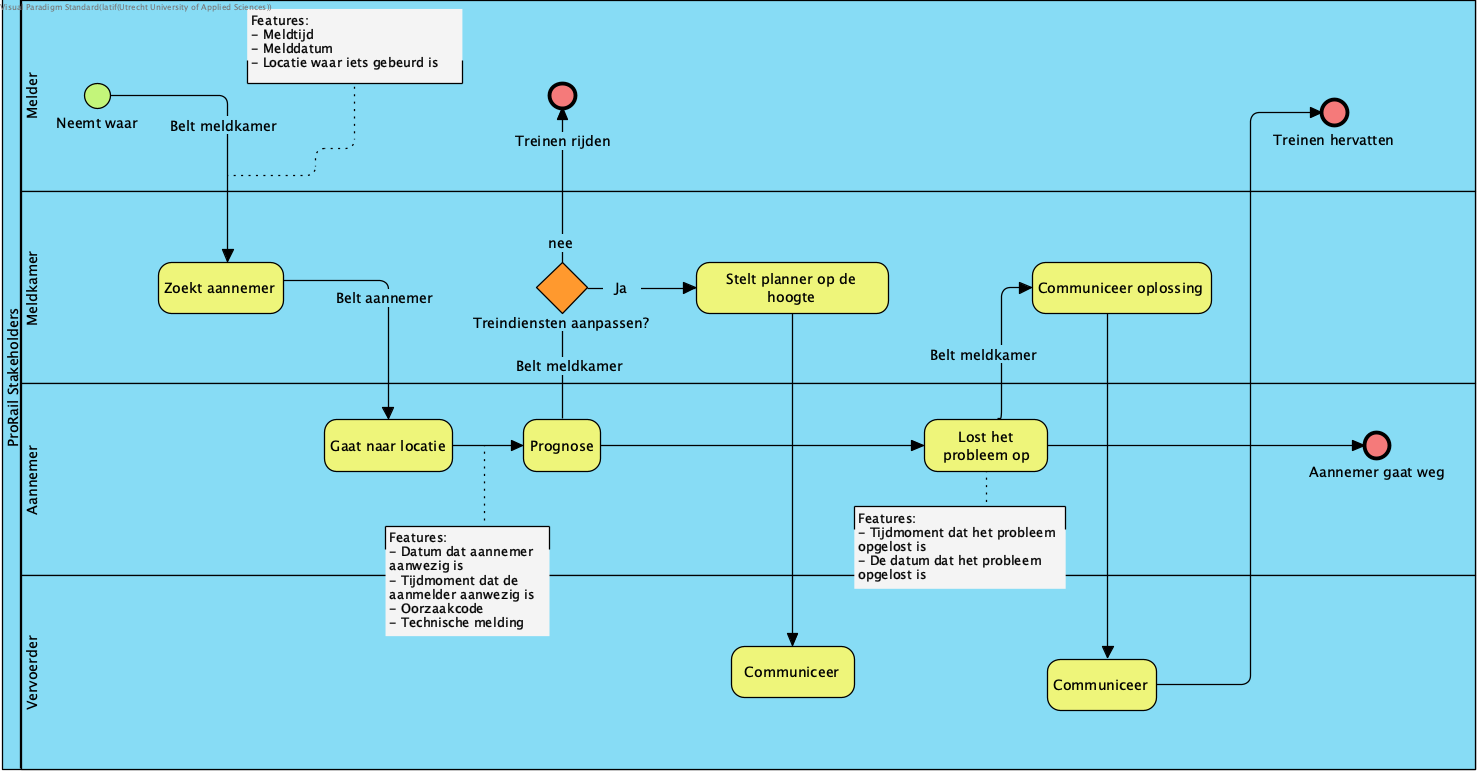
\includegraphics[width=10cm]{bpmn.png}
    \caption{BPMN (Business Process Model and Notation)}
\end{figure}

\subsection{Stakeholders}
Tijdens het project hebben we gekeken naar wie er allemaal betrokken zijn bij het proces rondom een storing, en wie er dus belang hebben bij een betere manier van voorspellen. Deze belanghebbenden (oftewel stakeholders) zijn de mensen of partijen die direct of indirect geraakt worden door een storing, en dus ook baat hebben bij een goede oplossing. Omdat we te maken hebben met een groot proces met meerdere stappen en afdelingen, zijn er best veel belanghebbenden.

\begin{itemize}
    \item \textbf{Meldkamer van ProRail:} Hier begint het hele proces. De meldkamer ontvangt de melding van de storing en moet direct actie ondernemen. Ze schakelen een aannemer in en houden contact met alle betrokkenen. Voor hen is het handig om zo snel mogelijk te weten hoe lang iets ongeveer gaat duren, zodat ze kunnen schakelen.

    \item \textbf{Planners van ProRail:} Zodra een storing invloed heeft op het spoor, moeten planners beslissen of er een aangepaste dienstregeling nodig is. Hoe beter ze weten hoe lang een storing gaat duren, hoe beter ze dat kunnen inschatten. Zonder goede informatie is het vaak gokken, en dat zorgt voor extra overlast.

    \item \textbf{Aannemers:} De mensen die daadwerkelijk naar de storing toe gaan en het probleem oplossen. Zij geven belangrijke informatie door, zoals de oorzaak en wanneer ze ter plekke zijn. Deze info gebruiken wij in onze modellen om te voorspellen hoe lang het nog gaat duren.

    \item \textbf{Vervoerders:} Als een storing impact heeft op het treinverkeer, zijn de vervoerders daar de dupe van. Zij moeten hun treinen en personeel opnieuw inplannen en zorgen dat reizigers weten waar ze aan toe zijn. Hoe sneller zij weten wat de impact is, hoe sneller ze kunnen schakelen.

    \item \textbf{Reizigers:} De mensen die elke dag met de trein reizen. Zij hebben natuurlijk geen invloed op het proces, maar ze merken de gevolgen wel direct. Door betere voorspellingen kunnen we de vertraging voor hen zoveel mogelijk beperken en beter communiceren wat er aan de hand is.

    \item \textbf{DataLab van ProRail:} Het DataLab is de afdeling binnen ProRail die zich bezighoudt met innovatie en data. Zij hebben ons gevraagd om dit project op te pakken. Ze willen weten of machine learning hierbij kan helpen, en of onze aanpak in de praktijk toegevoegde waarde biedt.

    \item \textbf{Ons projectteam (HU-studenten):} Tot slot zijn wij zelf ook belanghebbenden. Voor ons is het belangrijk dat het project duidelijk afgebakend is, dat de data bruikbaar is, en dat we goede feedback krijgen. Alleen dan kunnen wij iets maken wat echt gebruikt gaat worden.
\end{itemize}

\subsection{Knelpunten}
Tijdens het project kwamen we verschillende knelpunten tegen, zowel in het proces als in de data. Deze punten zorgen ervoor dat het moeilijk is om direct een goed werkend model of systeem te maken. Hieronder de belangrijkste knelpunten die we zijn tegengekomen:

\begin{itemize}
  \item \textbf{Inzicht in het proces:} In het begin was het onduidelijk hoe het proces precies verliep binnen ProRail. Omdat we extern zijn, wisten we niet wat er allemaal gebeurt vanaf het moment dat een storing gemeld wordt tot aan de oplossing. Daardoor was het lastig om te bepalen waar onze applicatie echt waarde kon toevoegen.
  \item \textbf{Datakwaliteit:} De data waarmee we werken is allesbehalve perfect. Er zitten veel lege velden in, foutieve of inconsistente waarden, en soms ontbreekt essentiële informatie. Dit maakt het moeilijk om betrouwbare voorspellingen te doen. Ook is de data erg technisch en soms lastig te interpreteren.
  \item \textbf{Tijdstip van datatoegang:} Niet alle informatie is meteen beschikbaar wanneer een storing net gemeld is. Sommige data komt pas later in het proces binnen, bijvoorbeeld als de aannemer ter plekke is. Daardoor kunnen we niet altijd meteen een goede voorspelling doen.
  \item \textbf{Complexiteit van het probleem:} Het voorspellen van de duur van een storing is lastig, omdat elke storing anders is. De ene keer is het een kapotte bovenleiding, de andere keer een wisselstoring. Er zijn veel factoren die invloed hebben, en die zijn lang niet altijd duidelijk of meetbaar.
  \item \textbf{Gebrek aan standaardisatie:} Veel waarden in de data zijn handmatig ingevoerd en worden niet altijd op dezelfde manier geregistreerd. Dit zorgt voor ruis in de data en bemoeilijkt het trainen van een goed model.
\end{itemize}

\newpage
\section{Data}

\subsection{Waar we mee werken}
Nu we weten hoe het hele proces verloopt, kunnen we ons gaan richten op misschien wel het belangrijkste deel van het project: de data. De voorspellingen die wij gaan doen, zijn volledig gebaseerd op deze data. Als we niet goed begrijpen hoe de data werkt, kunnen we geen betrouwbare modellen maken. Daarom hebben we grondig onderzocht wat er precies in de dataset staat en hoe deze past binnen de workflow van het bedrijf. Door het proces goed te begrijpen, kunnen we bepalen op welk moment in die workflow onze voorspellingen het meest van waarde zijn. Bijvoorbeeld: bij het eerste meldmoment is er nog weinig informatie beschikbaar, maar zodra de aannemer ter plaatse is, beschikken we over meer gegevens die het mogelijk maken om een nauwkeurige inschatting te geven van de hersteltijd.

\subsection{Het onderzoek}
Daarna zijn we ons gaan focussen op de inhoud van de dataset, aangezien dit de basis vormt van alles wat we gaan doen. We hebben te maken met een grote dataset van ongeveer 800.000 rijen vol storingsinformatie, bestaande uit tekstvelden, tijdstempels, numerieke waarden en categorische kenmerken. Tijdens de verkenning viel meteen op dat er veel dubbele rijen, lege velden en onlogische tijdswaarden aanwezig waren. Deze kunnen het leerproces van een model verstoren, dus zijn we kritisch gaan kijken naar welke informatie betrouwbaar en bruikbaar is. Door per kolom te analyseren hoe vaak waarden voorkomen, hoe logisch ze zijn en hoe ze zich verhouden tot andere velden, kregen we een goed beeld van de kwaliteit en structuur van de data.

\subsection{Opschonen van de data}
De volgende stap was het opschonen van de data, zodat deze geschikt is voor het bouwen van modellen. We hebben verschillende problemen ontdekt, zoals foutieve of ontbrekende waarden, en kolommen die volledig leeg of niet relevant zijn voor ons doel. Vooral kolommen die eindigen op \_gst bleken overbodig en zijn verwijderd. Vervolgens hebben we tijdvelden omgezet naar het aantal minuten sinds middernacht, zodat ze rekenkundig verwerkt konden worden. Daarnaast hebben we filters toegepast: storingen die korter dan 15 minuten of langer dan 8 uur duren zijn uitgesloten, omdat deze extreemwaarden het model negatief beïnvloeden. Ook zijn dubbele rijen verwijderd en foutieve prognosewaarden eruit gefilterd of gecorrigeerd waar mogelijk. Door deze stappen kregen we een schonere en betrouwbaardere dataset waarmee we verder konden.

\subsection{Analyse van de hersteltijd}
Om een beter beeld te krijgen van de verdeling van de hersteltijd hebben we verschillende visualisaties gemaakt. Hieronder kunnen we zien hoe de data zich gedraagt voordat en nadat we de extreme waarden hebben weggehaald.

\begin{figure}[H]
    \centering
    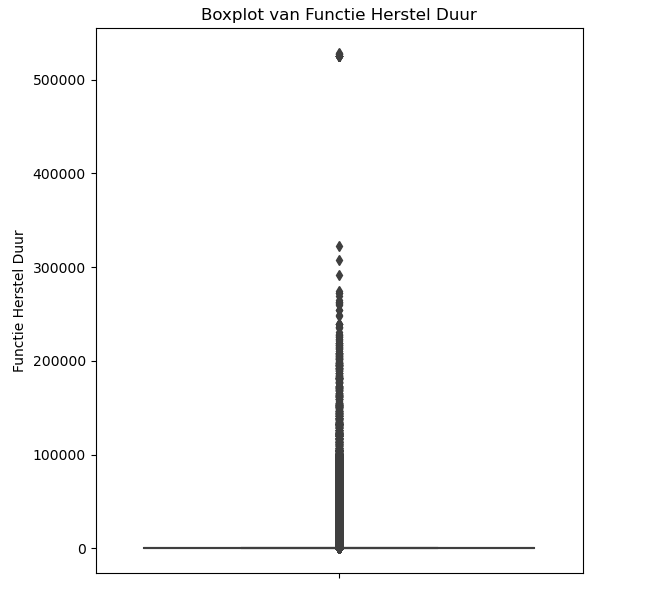
\includegraphics[width=10cm]{boxplot_FH_duur.png}
    \caption{Boxplot van de oorspronkelijke data - veel extreme waarden}
\end{figure}

\begin{figure}[H]
    \centering
    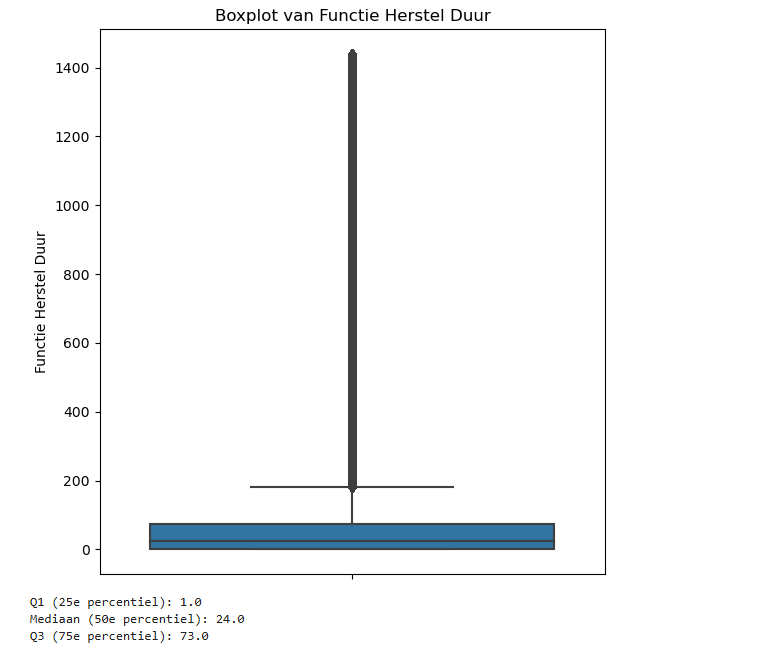
\includegraphics[width=10cm]{boxplot_target.png}
    \caption{Boxplot na het wegfilteren van extreme waarden - veel schonere verdeling}
\end{figure}

\begin{figure}[H]
    \centering
    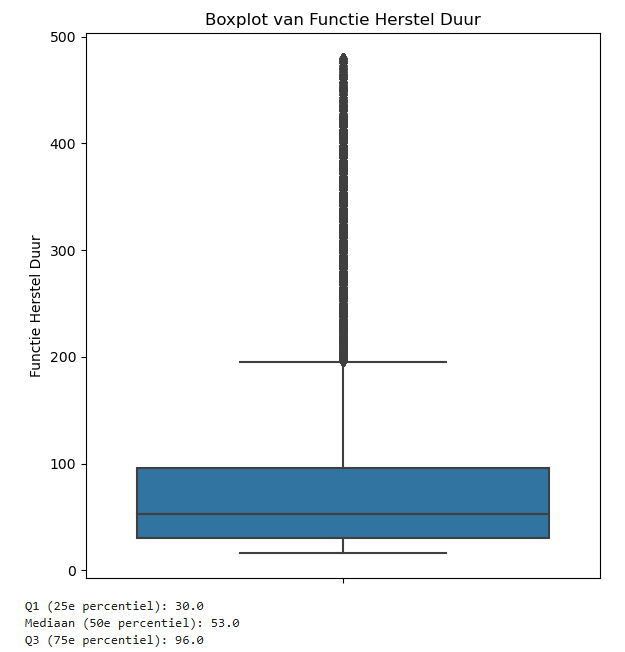
\includegraphics[width=10cm]{boxplot_target_filter.png}
    \caption{Boxplot van de definitieve dataset - klaar voor modeltraining}
\end{figure}

\subsection{Gekozen features}
Op het eerste gezicht zijn wij breed gaan kijken welke kolommen wij willen gebruiken. Uiteindelijk hebben we besloten om de volgende kolommen te gebruiken:
\begin{itemize}
  \item \textbf{stm\_sap\_melddatum}: De datum van de melding.
  \item \textbf{stm\_sap\_meldtijd}: De tijd van de melding.
  \item \textbf{stm\_aanntplj\_tijd}: De tijd dat de aannemer ter plaatse is. 
  \item \textbf{stm\_progfh\_in\_duur}: De prognose van de functie hersteltijd.
  \item \textbf{stm\_prioriteit}: De prioriteit van de storing.
  \item \textbf{stm\_oorz\_code}: De oorzaakcode waar de storing in valt.
  \item \textbf{stm\_contractgeb\_mld}: Het contractgebied van de melding.
  \item \textbf{stm\_techn\_mld}: Het techniekgebied van de melding.
\end{itemize}
Deze kolommen hebben we gekozen omdat ze het meest relevant zijn voor het voorspellen van de hersteltijd. Ons target, oftewel wat we willen voorspellen, is targetherstel. Dit is de tijd die het duurt vanaf het moment dat de aannemer aanwezig is tot het moment dat het incident verholpen is.

\subsection{Analyse per kenmerk}
Door de data per kenmerk te analyseren, krijgen we inzicht in welke factoren de grootste invloed hebben op de hersteltijd. Hieronder kunnen we zien hoe de gemiddelde hersteltijd varieert per contractgebied, geografische locatie, oorzaakcode en prioriteit.

\begin{figure}[H]
    \centering
    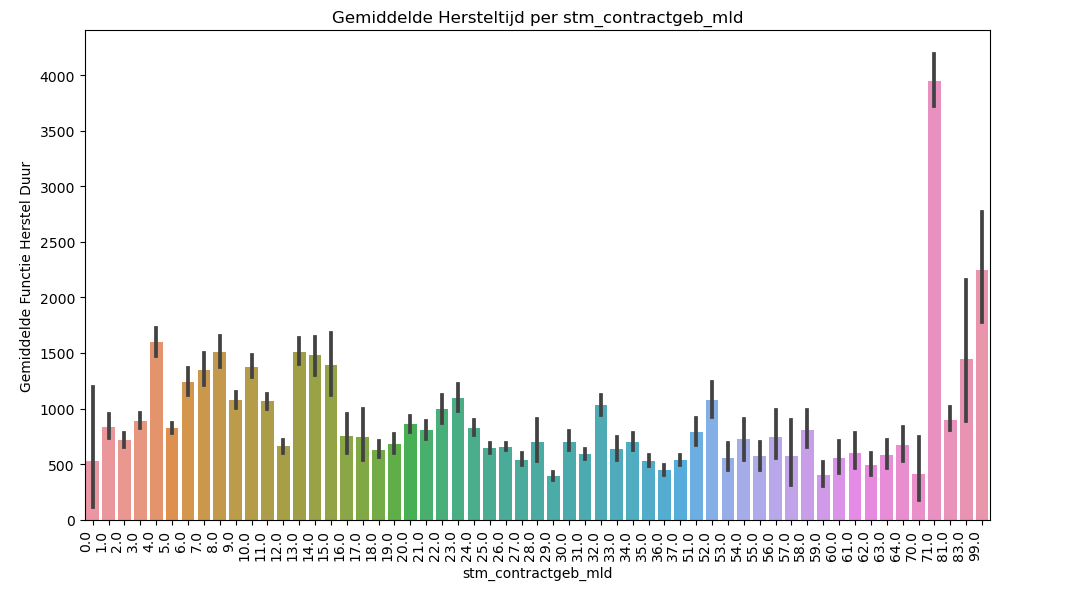
\includegraphics[width=12cm]{contractgeb.png}
    \caption{Gemiddelde hersteltijd per contractgebied - duidelijke verschillen tussen regio's}
\end{figure}

\begin{figure}[H]
    \centering
    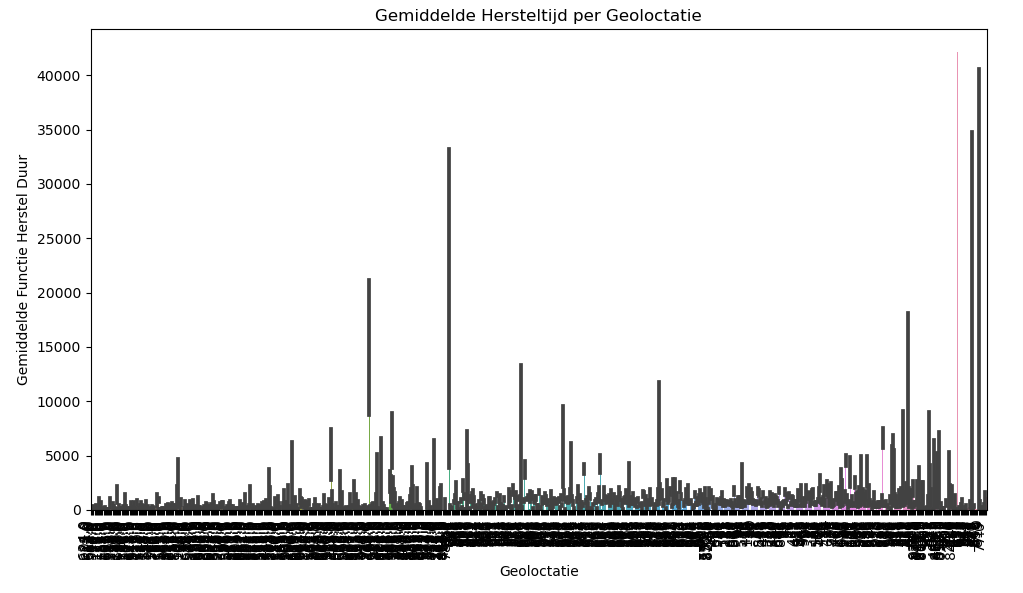
\includegraphics[width=12cm]{Geo.png}
    \caption{Gemiddelde hersteltijd per geografische locatie - grote spreiding in het land}
\end{figure}

\begin{figure}[H]
    \centering
    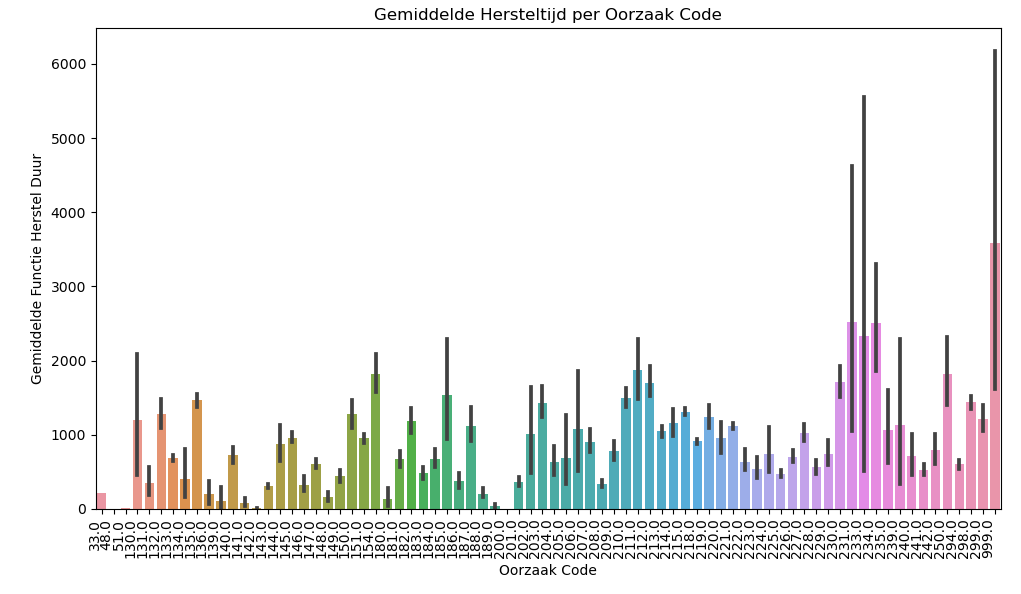
\includegraphics[width=12cm]{oorzakcode.png}
    \caption{Gemiddelde hersteltijd per oorzaakcode - verschillende typen storingen variëren sterk}
\end{figure}

\begin{figure}[H]
    \centering
    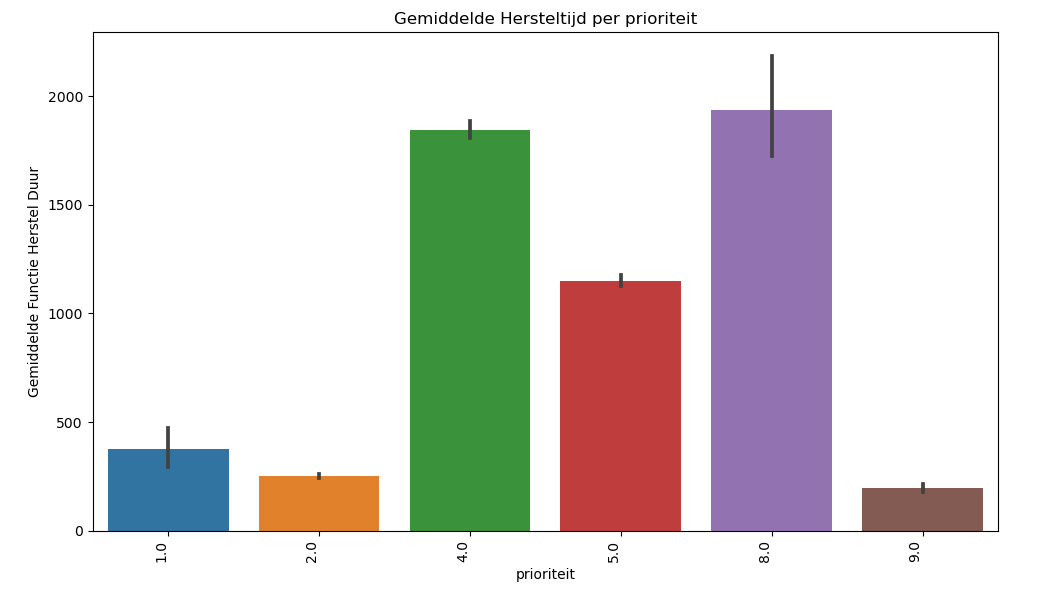
\includegraphics[width=12cm]{priorteit.png}
    \caption{Gemiddelde hersteltijd per prioriteit - hogere prioriteit niet altijd sneller opgelost}
\end{figure}

\subsection{Voorspeltarget}
Nu we weten welke data we gebruiken, is het tijd om te kijken naar wat we precies willen voorspellen. In ons geval is dat de hersteltijd van een storing, vanaf het moment dat de aannemer aanwezig is. Dit noemen we het target, en die kolom heet targetherstel. Deze waarde geeft aan hoeveel minuten het duurt vanaf aankomst tot volledige oplossing van de storing. Bij het analyseren van deze target zagen we dat 25\% van de storingen binnen 10 minuten opgelost is, terwijl sommige gevallen juist dagen of zelfs maanden duren. Om te voorkomen dat deze extremen de prestaties van het model verstoren, hebben we storingen onder de 15 minuten en boven de 8 uur uitgesloten.

\newpage
\section{Modellen}

\subsection{Lineaire regressie}
Als eerste hebben we een lineair regressiemodel toegepast. Dit model probeert de hersteltijd te voorspellen door een rechte lijn te trekken door de data, waarbij elke feature een lineaire bijdrage levert aan de uitkomst. Het voordeel van lineaire regressie is dat het eenvoudig en snel te trainen is, en dat het makkelijk te interpreteren is. Toch zagen we dat de prestaties beperkt bleven, vooral omdat het model moeite had met het vangen van niet-lineaire verbanden in de data. De R²-waarde was lager dan verwacht en de voorspellingen verbeterden slechts licht ten opzichte van de baseline.

\subsection{Decision Tree}
Vervolgens hebben we een decision tree model gebruikt. Dit model splitst de data stapsgewijs op basis van de belangrijkste kenmerken, waardoor het complexe, niet-lineaire relaties kan vangen. De boom verdeelde de hersteltijd in tijdsklassen van ongeveer 15 minuten, wat hielp om specifieke groepen storingen beter te onderscheiden. Dit resulteerde in een verbetering van de nauwkeurigheid en een lagere RMSE ten opzichte van lineaire regressie. Een nadeel was dat het model geneigd was tot overfitting, waardoor het minder goed generaliseerde naar nieuwe data.

\subsection{Random Forest}
Als laatste hebben we een Random Forest model getraind, wat eigenlijk een verzameling van meerdere decision trees is. Door het combineren van verschillende bomen vermindert het model overfitting en verbetert het de robuustheid van de voorspellingen. Met geoptimaliseerde hyperparameters leverde het Random Forest model de beste resultaten: een lagere RMSE en een hogere nauwkeurigheid dan de voorgaande modellen. Toch bleef er ruimte voor verbetering, vooral op het gebied van coverage, oftewel het betrouwbaar voorspellen van een breed scala aan storingsgevallen.

\section{Resultaten van de modellen}
De modellen zijn beoordeeld op basis van root mean squared error (RMSE), accuracy binnen een tolerantie van ±15 minuten, en coverage, het percentage voorspellingen dat een betrouwbare inschatting gaf.

Het baseline model behaalde een accuracy van ongeveer 35\%, waarbij voorspellingen vaak de hersteltijd overschatten. Lineaire regressie verbeterde de accuracy iets naar circa 42\%, maar had nog steeds moeite met het modelleren van complexe patronen. Decision Trees lieten een verdere verbetering zien in zowel RMSE als accuracy, maar waren gevoelig voor overfitting.

Het Random Forest model presteerde het beste, met een accuracy die ruim 10\% hoger lag dan de baseline, de huidige menselijke prognose, en een duidelijk lagere RMSE. Dit betekent dat het model beter in staat is om de hersteltijd nauwkeurig te voorspellen dan de standaard inschattingen die nu worden gebruikt. Toch bleek dat ongeveer 80\% van de voorspellingen nog steeds de hersteltijd overschatte, wat aangeeft dat het model voorzichtig moet worden ingezet. De resultaten tonen aan dat er duidelijke vooruitgang is geboekt, maar dat verdere optimalisatie nodig is om betrouwbare en bruikbare voorspellingen te garanderen in de praktijk.

\newpage
\section{Applicatie}

\subsection{Ontwerp van de applicatie}
Het model waarin de voorspelling wordt gemaakt is erg ingewikkeld en vereist technische kennis. Daarom is er een applicatie gemaakt waarin je op een gebruiksvriendelijke manier hetzelfde resultaat kunt behalen. Omdat een goede applicatie maken veel werk kost, zijn wij als eerste visuele en interactieve ontwerpen gaan maken om te laten zien hoe de applicatie eruit gaat zien. We hebben wireframes en prototypes gemaakt om het ontwerp te testen. De applicatie moet simpel in ontwerp zijn, zodat gebruikers zonder technische achtergrond ermee kunnen werken.

\subsection{Implementatie en veiligheid}
Nadat dit getest is, zijn wij begonnen met het uitwerken van de applicatie, die vervolgens op het web geplaatst wordt zodat de betrokkenen er altijd bij kunnen. Omdat de applicatie online staat, hebben wij ons ook gefocust op de veiligheid, en is het dus niet toegankelijk voor iedereen. Er is een systeem gebouwd dat ervoor zorgt dat alleen de mensen met een account er toegang toe hebben.

\subsection{Werking van de applicatie}
De applicatie bestaat uit drie onderdelen: Voor de veiligheid is er een registratie en login pagina. Dit is er om de veiligheid te waarborgen, zodat alleen de medewerkers erbij kunnen. Als je eenmaal ingelogd bent, kom je op het dashboard terecht, waar de voorspellingen gemaakt worden. Hier vul je de benodigde data in, zodat je daarna een geschatte hersteltijd terugkrijgt. De lineaire regressie laat de tijd in enkele minuten zien, en de random forest laat het in tijdsloten van 15 minuten zien. Daarnaast heb je nog de oude voorspellingen die je terug kunt krijgen. Daar kun je ook data terugkrijgen zodat je vergelijkbare storingen terugkrijgt.

\newpage
\section{Conclusie}

Dit project heeft aangetoond dat het mogelijk is om machine learning in te zetten voor het voorspellen van hersteltijden van storingen in het spoorwegnet. Door de samenwerking met ProRail hebben wij een goed beeld gekregen van hun werkproces en de uitdagingen waar ze dagelijks mee te maken hebben. Het was belangrijk om eerst te snappen hoe het hele proces verloopt, voordat we aan de slag gingen met de data en modellen.

De data die we hebben gebruikt was complex en verre van perfect. Met bijna 900.000 rijen en 139 kolommen was het een behoorlijke klus om dit op te schonen en bruikbaar te maken. Na het wegfilteren van irrelevante informatie en het corrigeren van fouten, konden we uiteindelijk werken met een dataset die geschikt was voor het trainen van modellen. Dit proces heeft ons veel geleerd over hoe belangrijk datakwaliteit is voor het succes van een machine learning project.

Van de drie modellen die we hebben getest, presteerde het Random Forest model het beste met een RMSE van 55.03 en een accuracy van 42.31\%. Alle modellen scoorden beter op RMSE dan de baseline (69.40). De lineaire regressie behaalde een vergelijkbare accuracy als een menselijke prognose, maar bleef onder de baseline accuracy van 35.10\%. De Decision Tree en Random Forest modellen presteerden beter op zowel RMSE als accuracy, maar de coverage daalde van 81.39\% naar ongeveer 71\%. Dit betekent dat de modellen wel nauwkeuriger zijn wanneer ze een voorspelling doen, maar dat ze in minder gevallen een betrouwbare inschatting kunnen geven dan de huidige methode.

De applicatie die we hebben ontwikkeld maakt het mogelijk om deze voorspellingen op een gebruiksvriendelijke manier te gebruiken. Door een simpel ontwerp en een veilig inlogsysteem kunnen medewerkers van ProRail nu snel een inschatting krijgen van hoe lang een storing gaat duren. Dit helpt hen om betere beslissingen te nemen over het inzetten van aannemers en het aanpassen van de dienstregeling.

Hoewel de resultaten veelbelovend zijn, is dit nog geen perfecte oplossing. Het model moet nog verder geoptimaliseerd worden en er moet meer gekeken worden naar hoe het in de praktijk gebruikt gaat worden. Ook zou het interessant zijn om in de toekomst meer data te verzamelen en andere algoritmes uit te proberen. Maar dit project laat wel zien dat data-driven beslissingen nemen bij ProRail zeker mogelijk is en dat er nog veel te winnen valt door slimmer om te gaan met de beschikbare informatie.

\end{document}
